\documentclass[11pt,a4paper,titlepage,oneside]{article}
\usepackage{LabProtocol}

\exercise{Exercise III}

% enter your data here
\groupno{6}
\authors{
  Thomas Scharinger, Matr. Nr. 11777710 \par
  {\small e11777710@student.tuwien.ac.at} \par
  Fabian Philipp Posch, Matr. Nr. 01456625 \par
  {\small e0123456@student.tuwien.ac.at} \par
  Maximilian Engl, Matr. Nr. 11775811 \par
  {\small e11775811@student.tuwien.ac.at}
}


\begin{document}

\maketitle

%%%%%%%%%%%%%%%%%%%%%%%%%%%%%%%%%%%%%%%%%%%%%%%%%%%%%%%%%%%%%%%%%%%%%%%%%%%%%%%%
%%%%%%%%%%%%%%%%%%%%%%%%%%%%%%%%%%%%%%%%%%%%%%%%%%%%%%%%%%%%%%%%%%%%%%%%%%%%%%%%

\begin{figure}[ht!]
  \centering
  \framebox[\linewidth]{
    %\rotatebox{30}{Insert your figure here.}
  }
  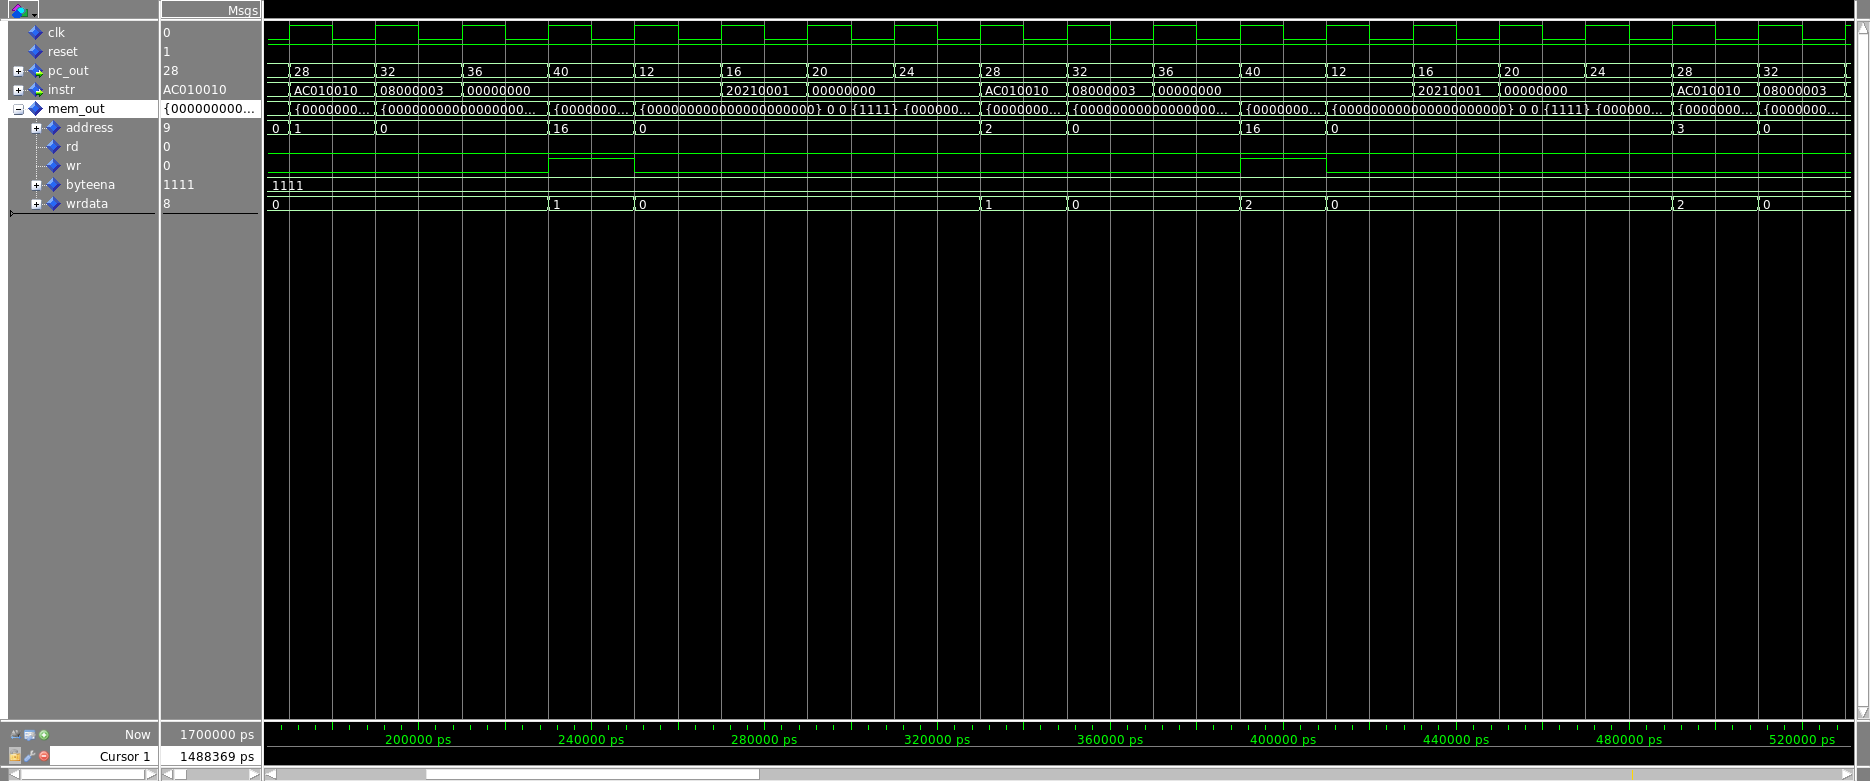
\includegraphics[width=1.0\linewidth]{p1.png}
  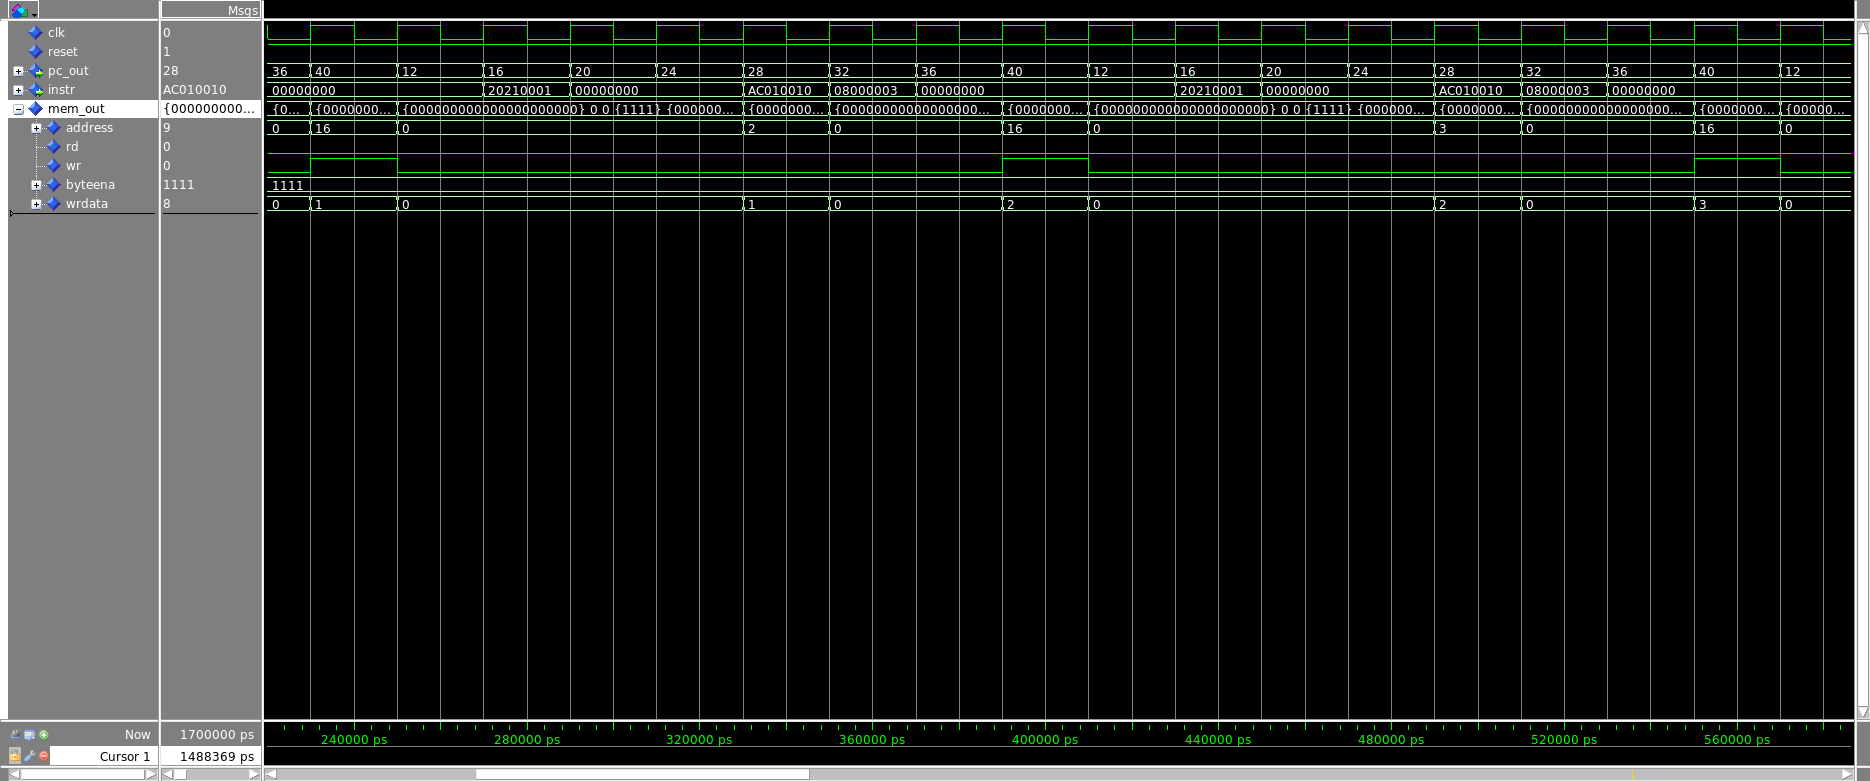
\includegraphics[width=1.0\linewidth]{p2.png}
  \caption{Simulation screenshot for Listing~\ref{lst:asmnofwd}.}
  \label{fig:sim}
\end{figure}

Make sure the following signals are visible in Figure~\ref{fig:sim} and the signal values are readable:
the program counter in the fetch stage, the instruction being fetched,
and the fields \texttt{address}, \texttt{rd}, \texttt{wr},
\texttt{byteena}, and \texttt{wrdata} in the \texttt{mem\_out} signal
coming out of the pipeline.

\begin{lstlisting}[language=,mathescape=false,float=ht,caption={Assembler example without forwarding},label=lst:asmnofwd]
        addi $1, $0, 0
        nop
        nop
loop:
        addi $1, $1, 1
        nop
        nop
        sw $1, 16($0)
        j loop
        nop
        nop
        nop
\end{lstlisting}
%%%%%%%%%%%%%%%%%%%%%%%%%%%%%%%%%%%%%%%%%%%%%%%%%%%%%%%%%%%%%%%%%%%%%%%%%%%%%%%%
%%%%%%%%%%%%%%%%%%%%%%%%%%%%%%%%%%%%%%%%%%%%%%%%%%%%%%%%%%%%%%%%%%%%%%%%%%%%%%%%

\end{document}
